% !TEX root = slides.tex

\section{Introduction}

\begin{frame}{Introduction}
    \only<1>{
        \begin{figure}
            \centering
            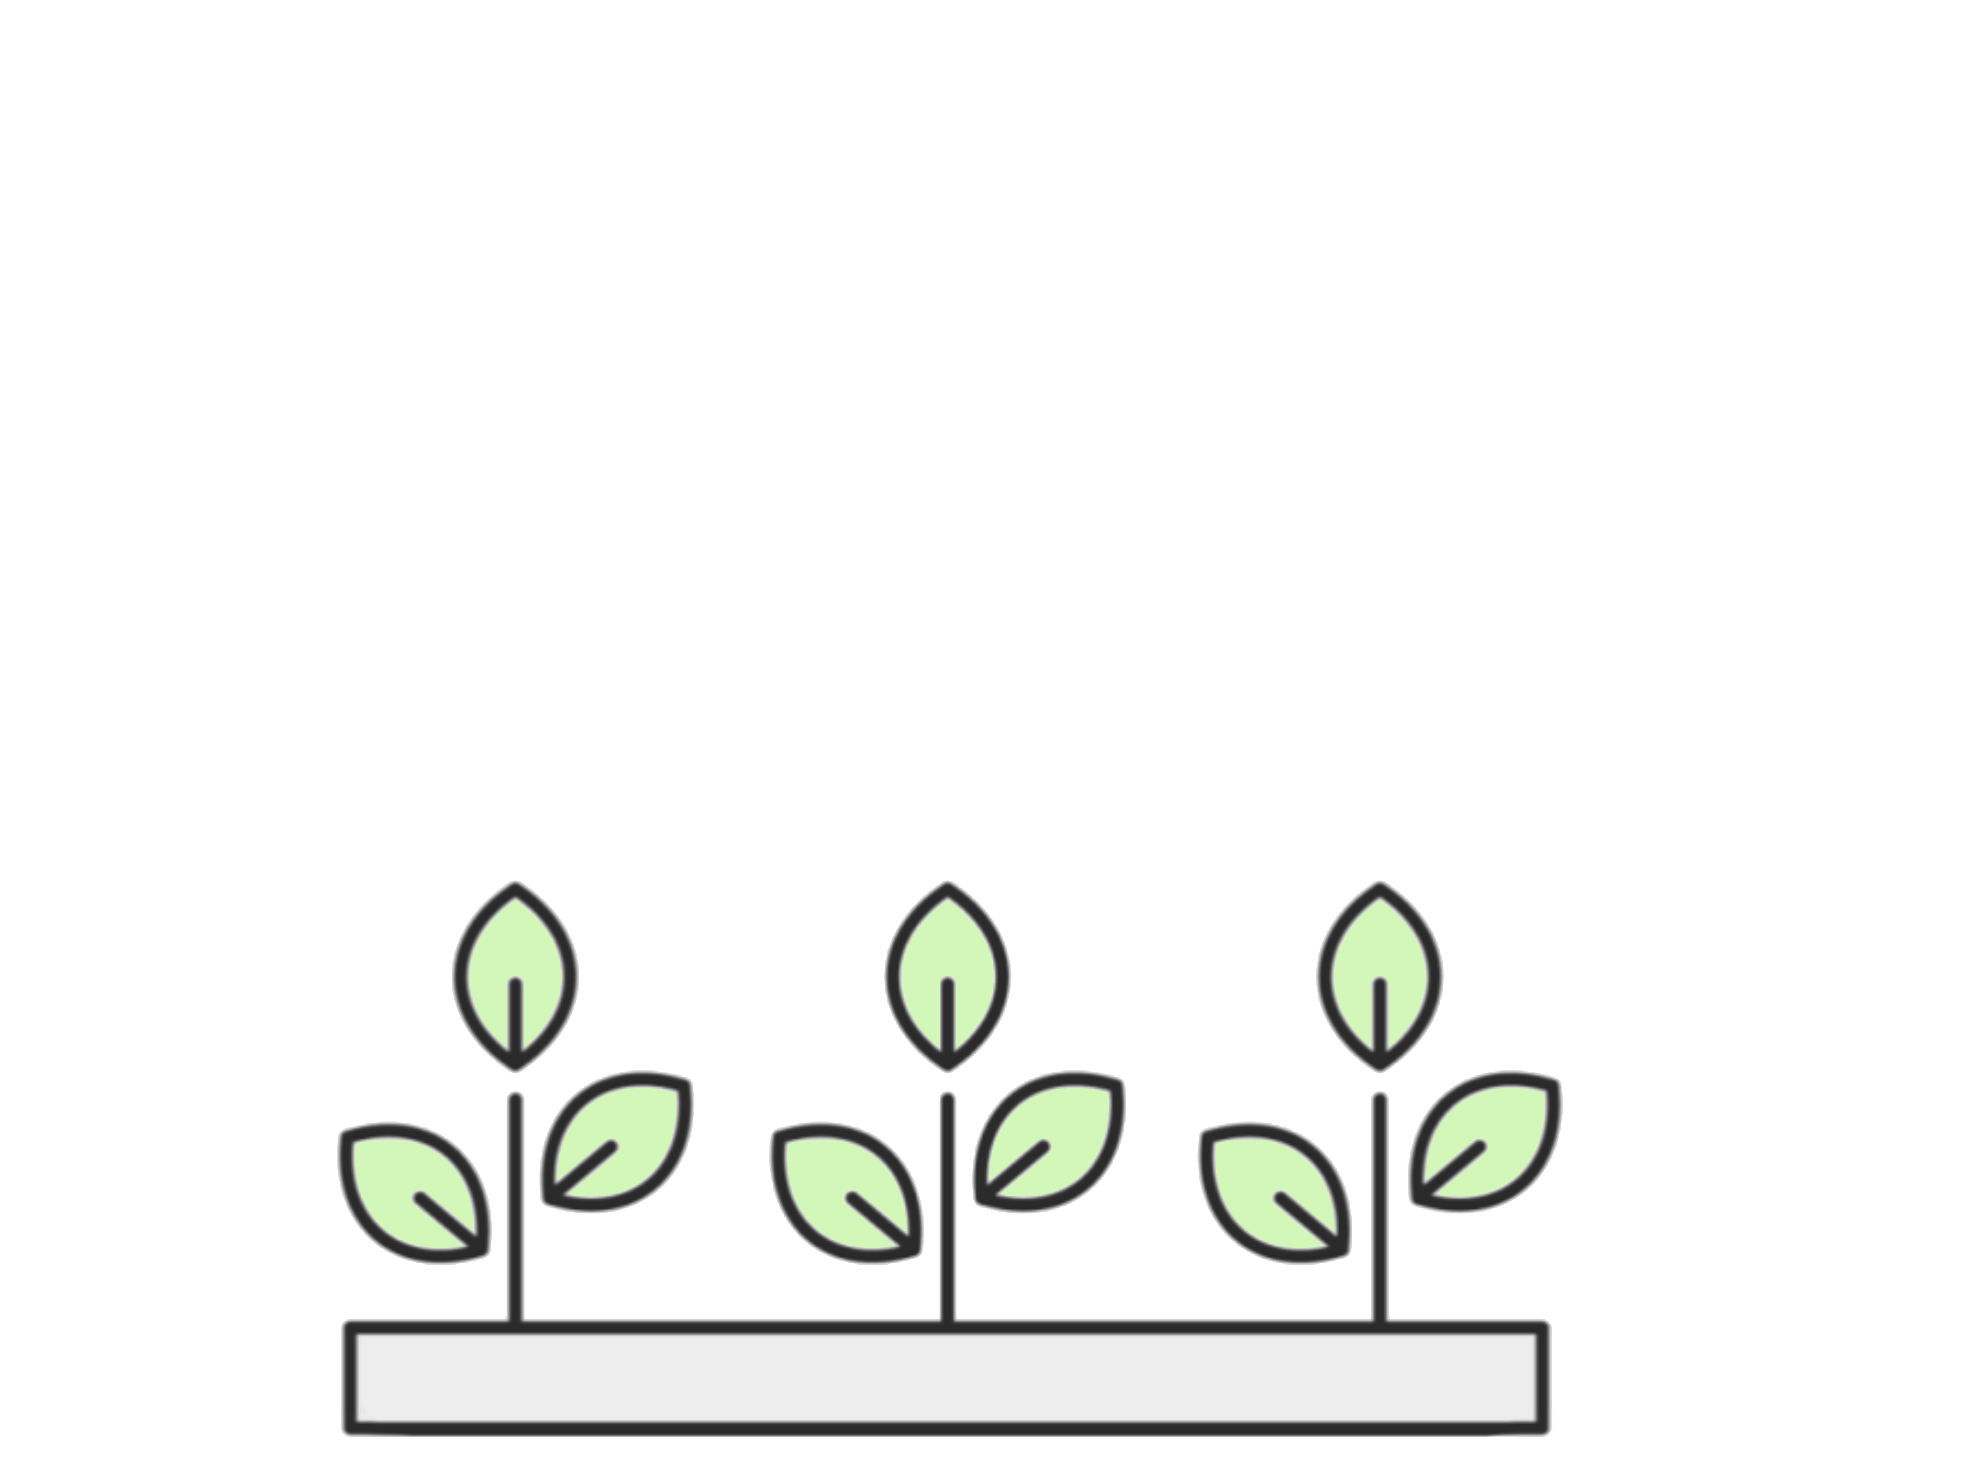
\includegraphics[scale=0.2]{figures/1_plants.png}
        \end{figure}
    }
    \only<2>{
        \begin{figure}
            \centering
            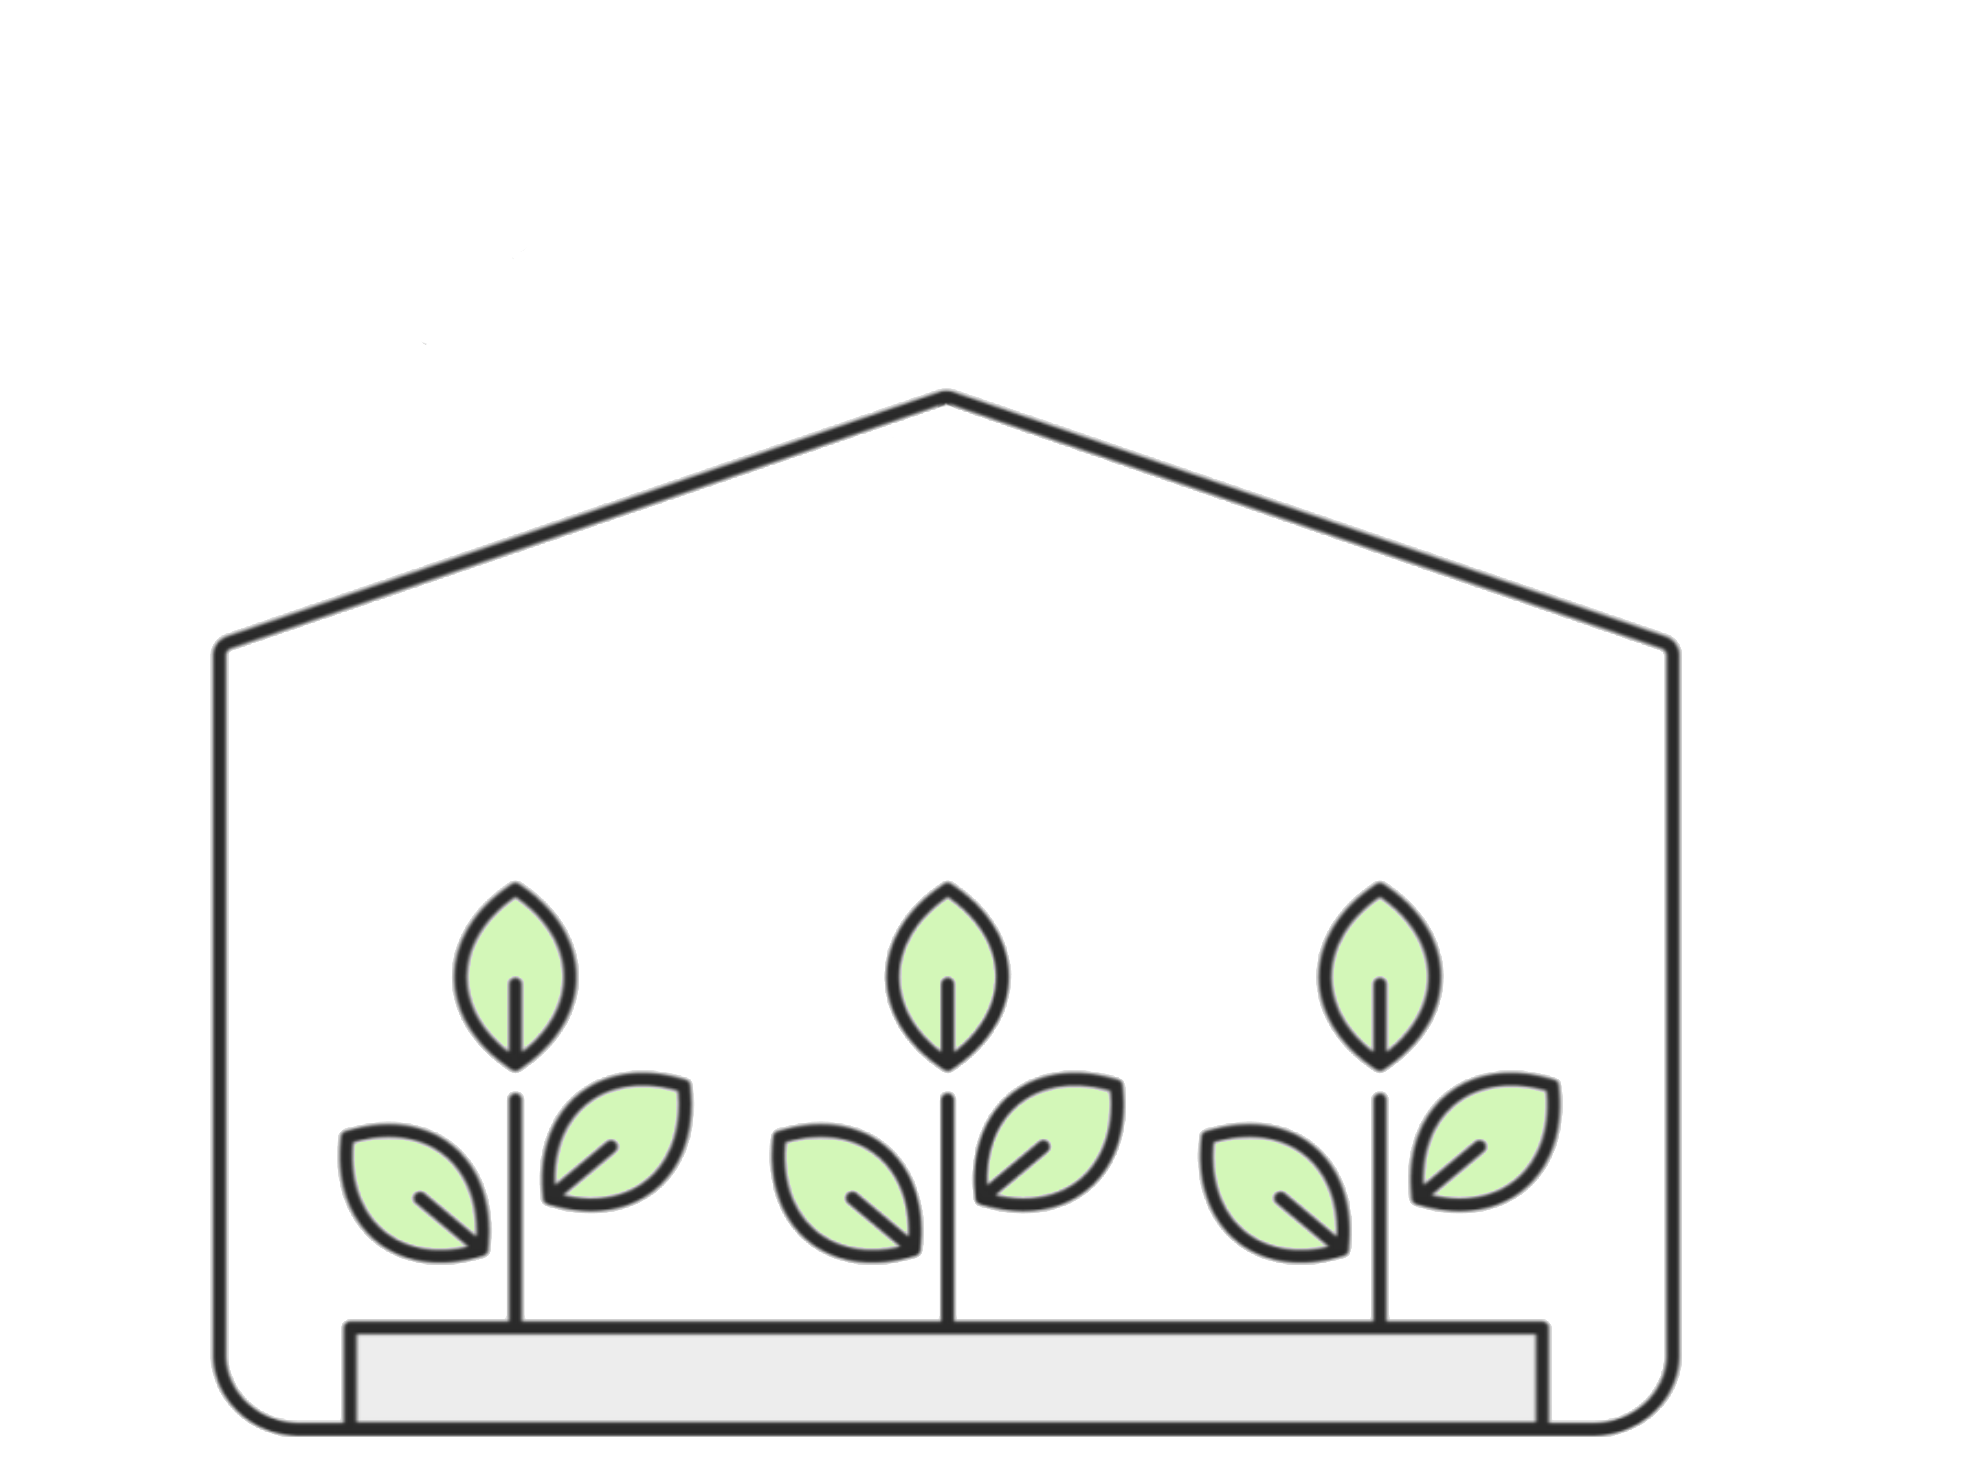
\includegraphics[scale=0.2]{figures/2_greenhouse.png}
        \end{figure}
    }
    \only<3>{
        \begin{figure}
            \centering
            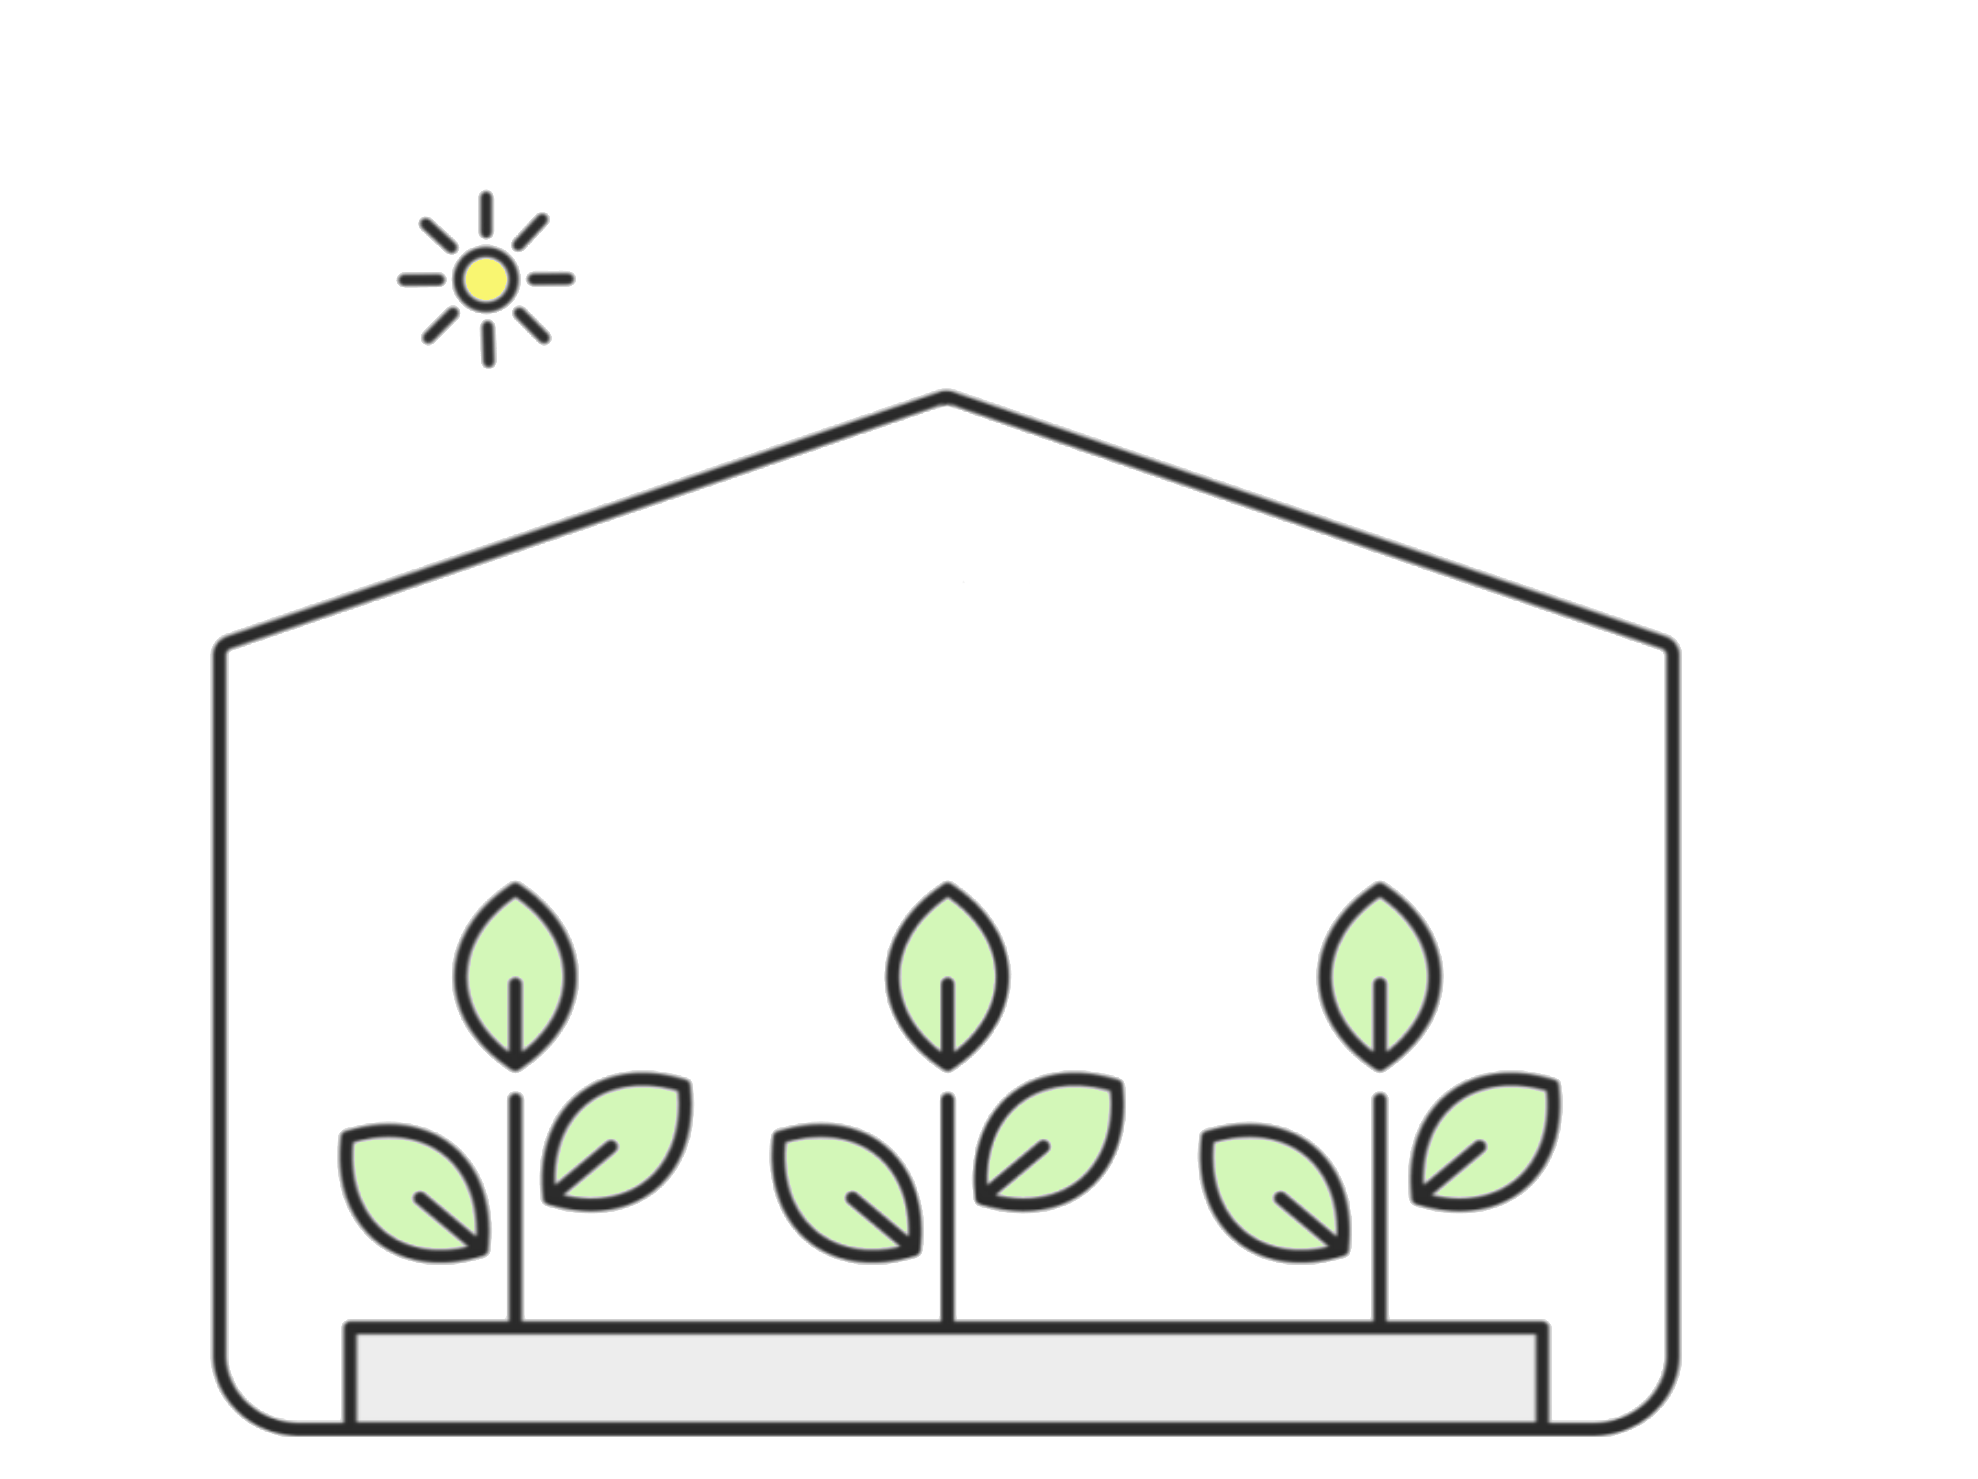
\includegraphics[scale=0.2]{figures/3_sun.png}
        \end{figure}
    }
    \only<4>{
        \begin{figure}
            \centering
            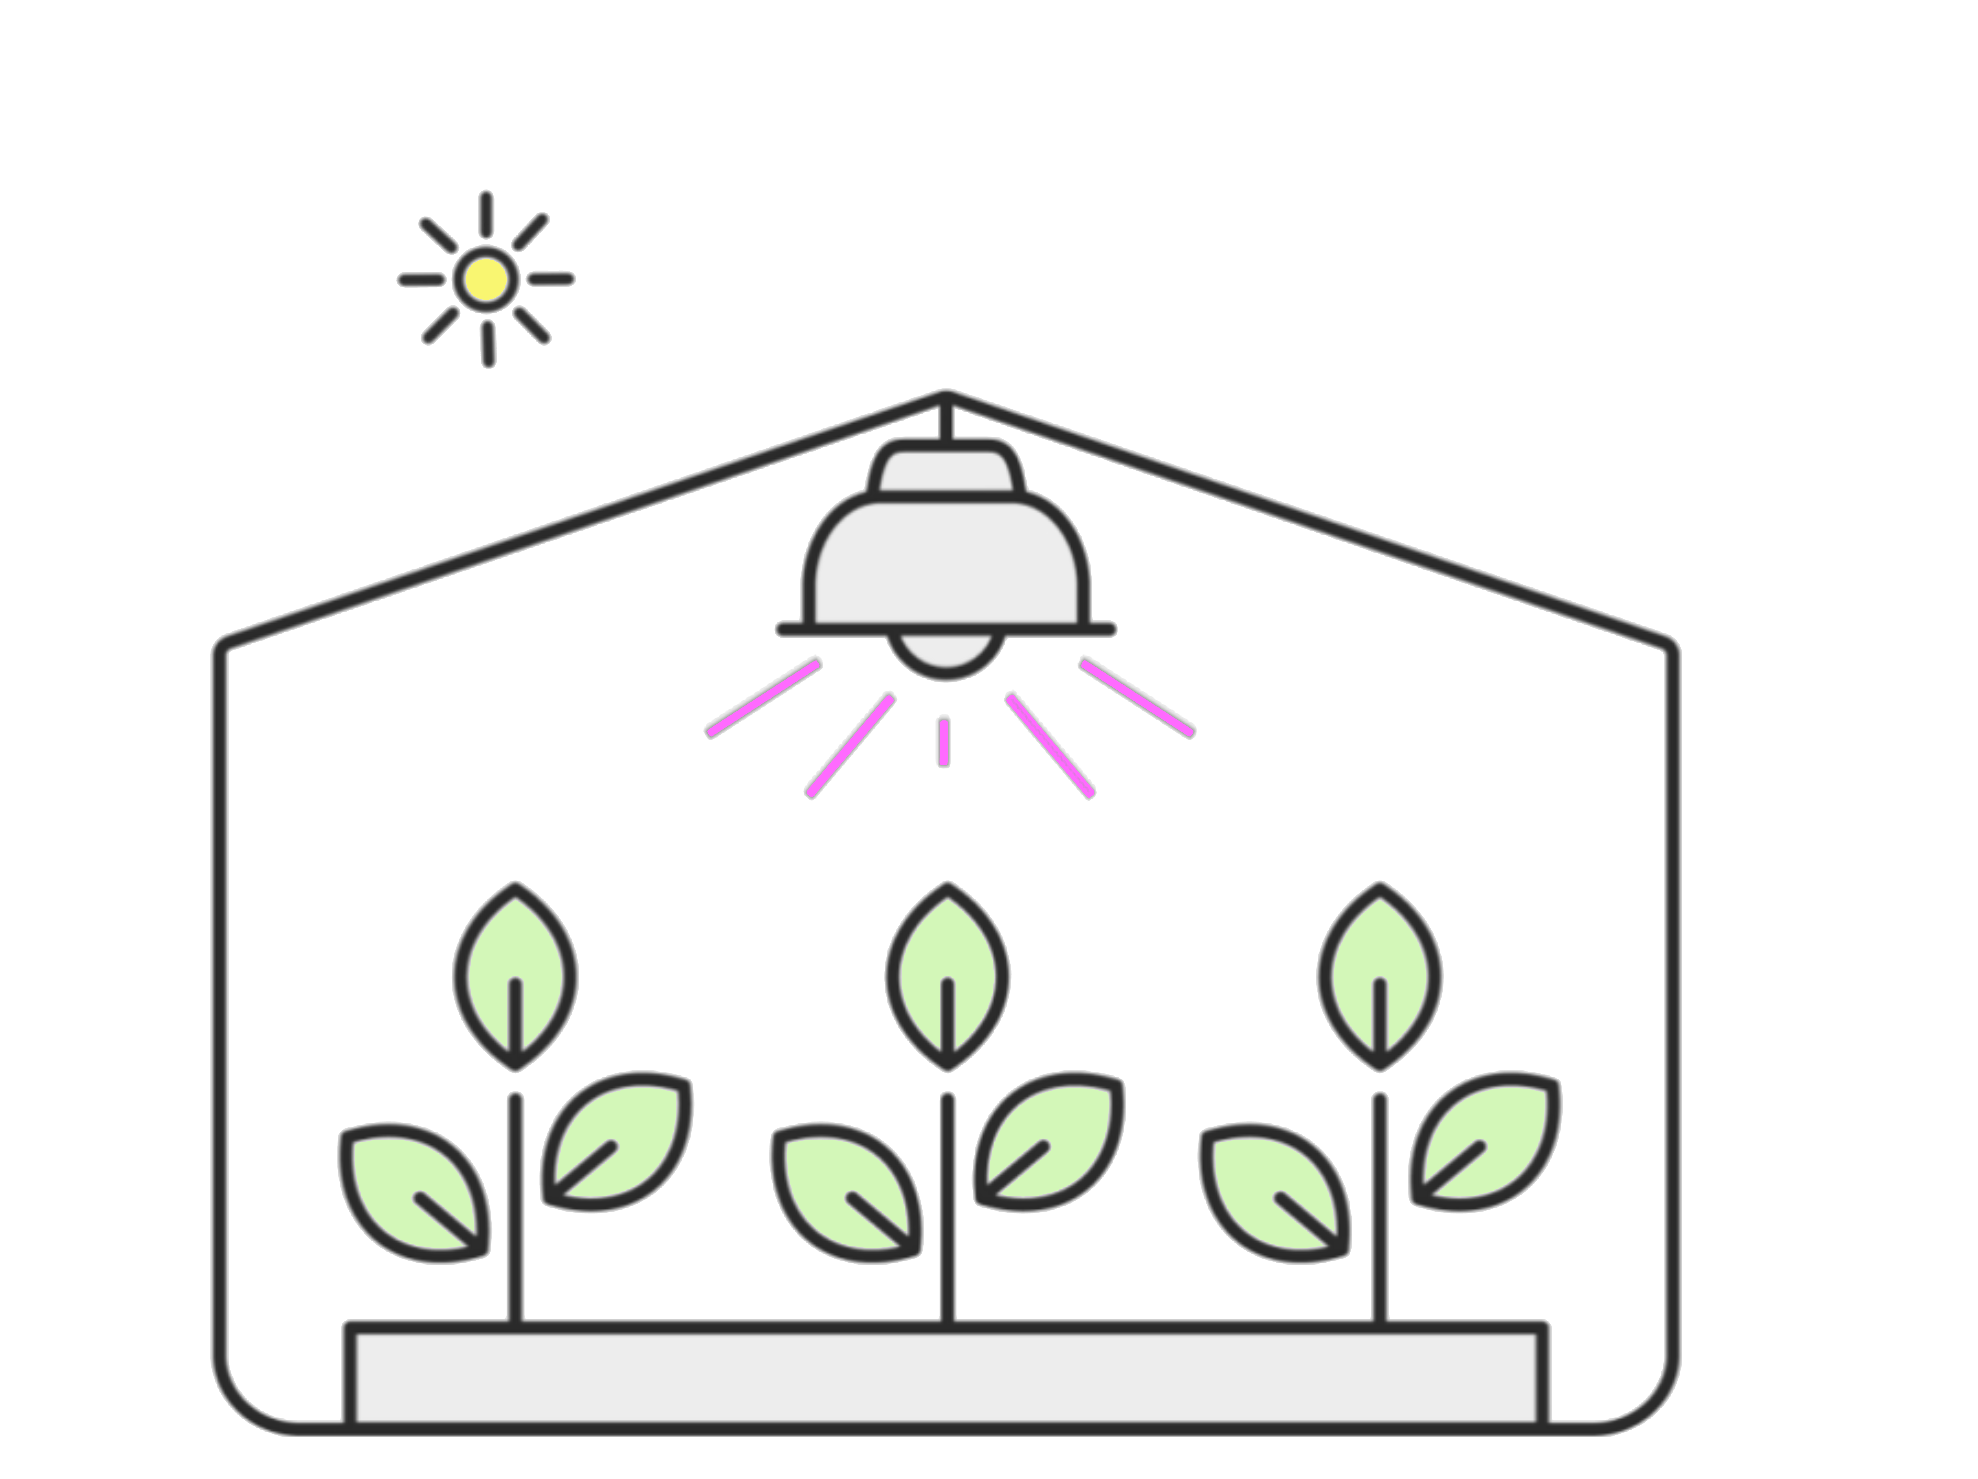
\includegraphics[scale=0.2]{figures/4_lights.png}
        \end{figure}
    }
    \only<5>{
        \begin{figure}
            \centering
            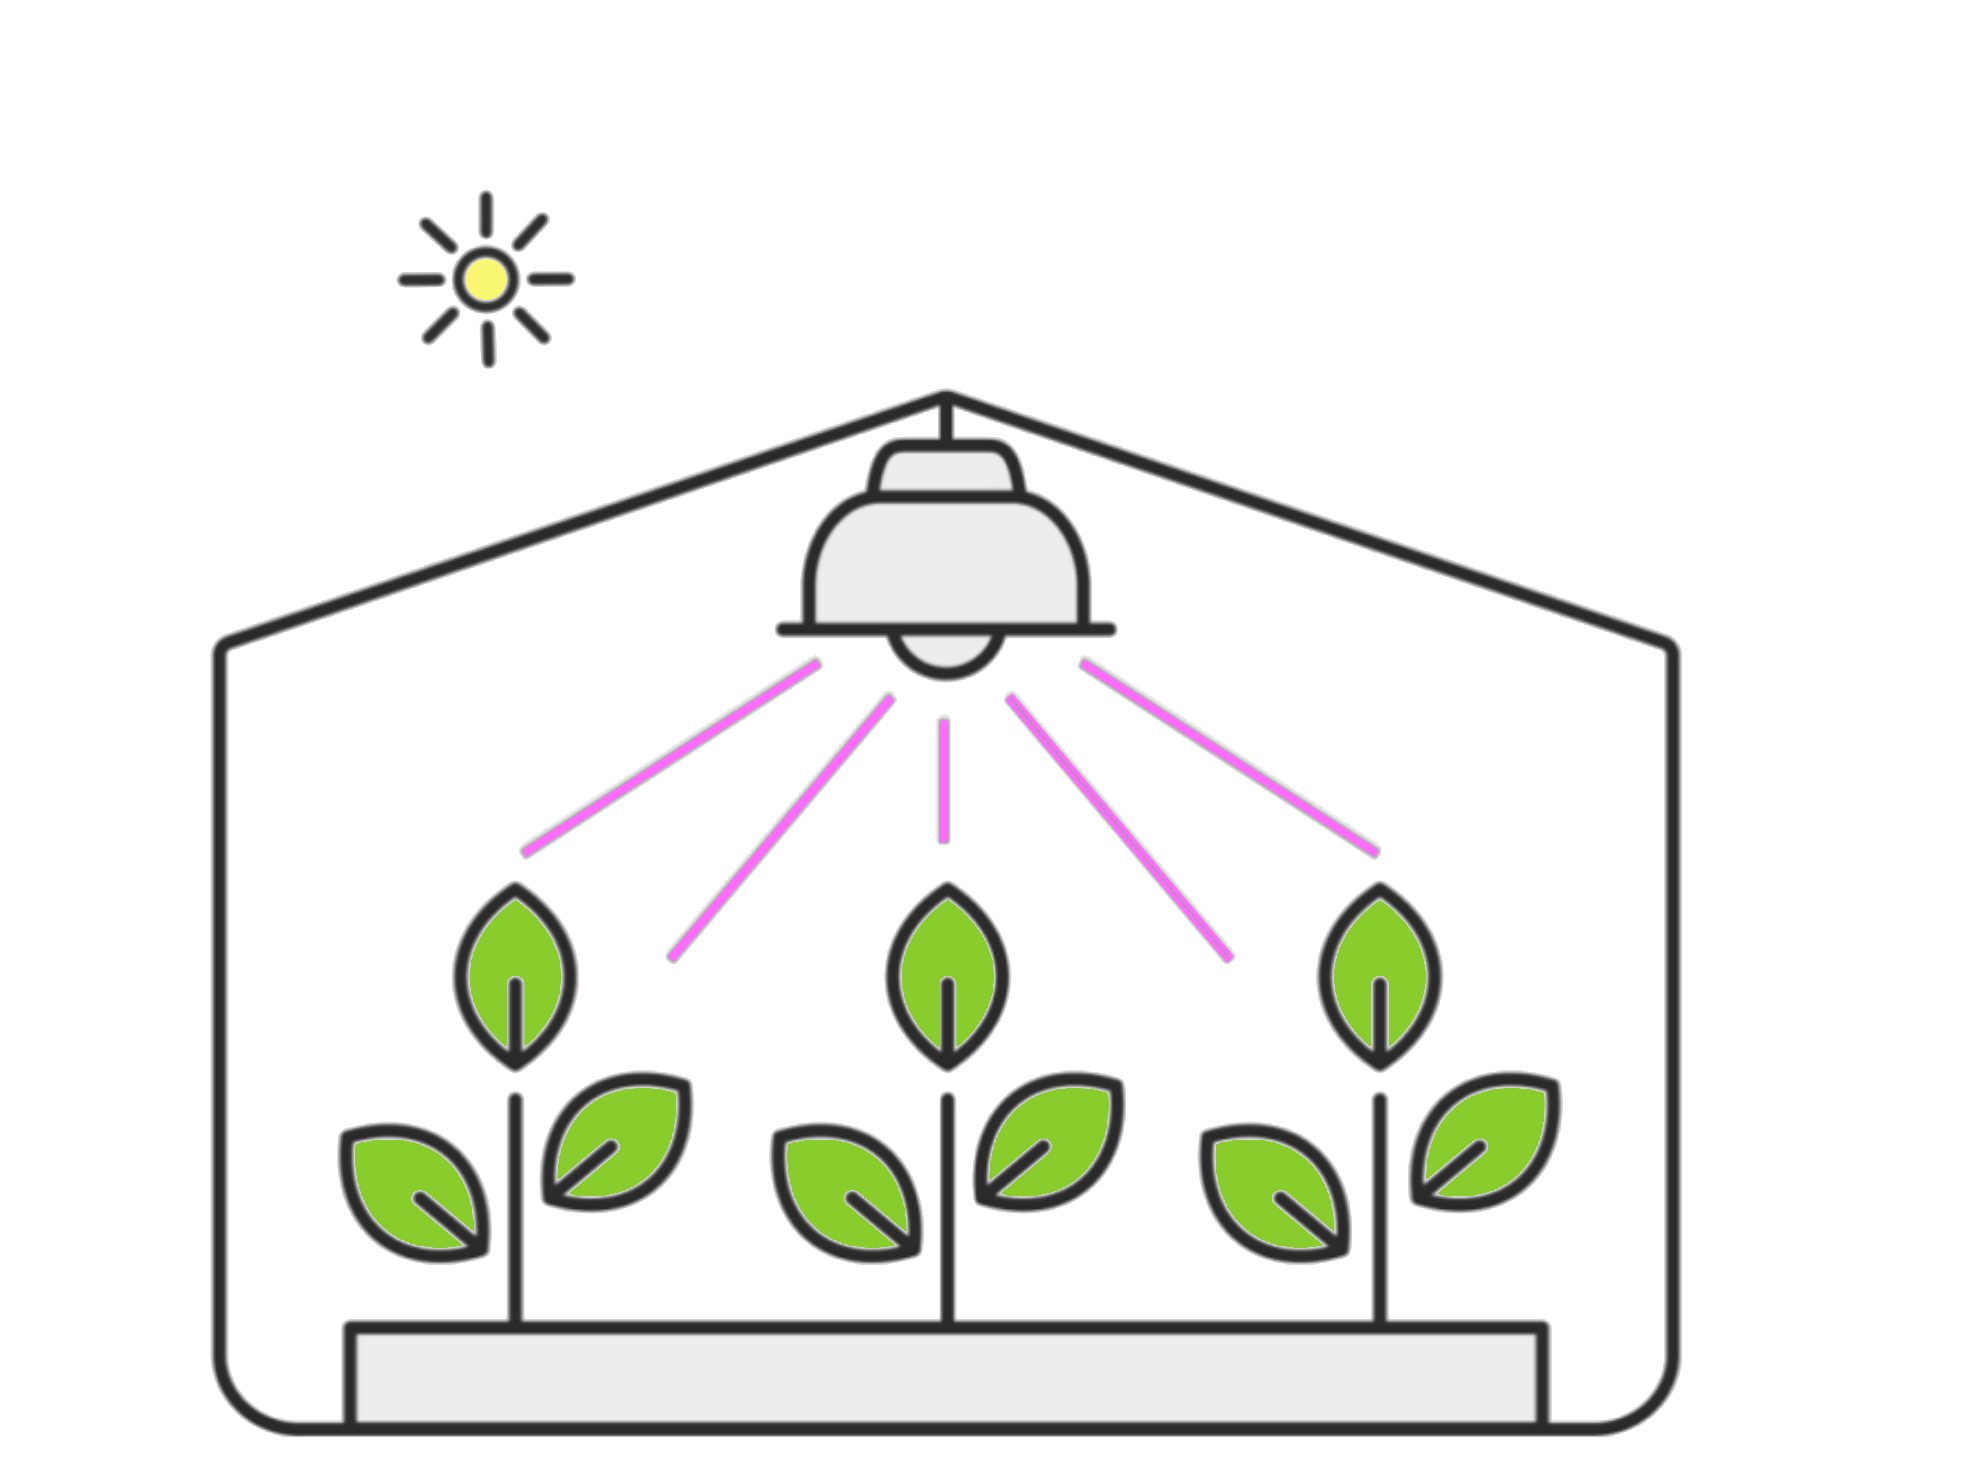
\includegraphics[scale=0.2]{figures/5_photosynthesis.png}
        \end{figure}
    }
    \only<6>{
        \begin{figure}
            \centering
            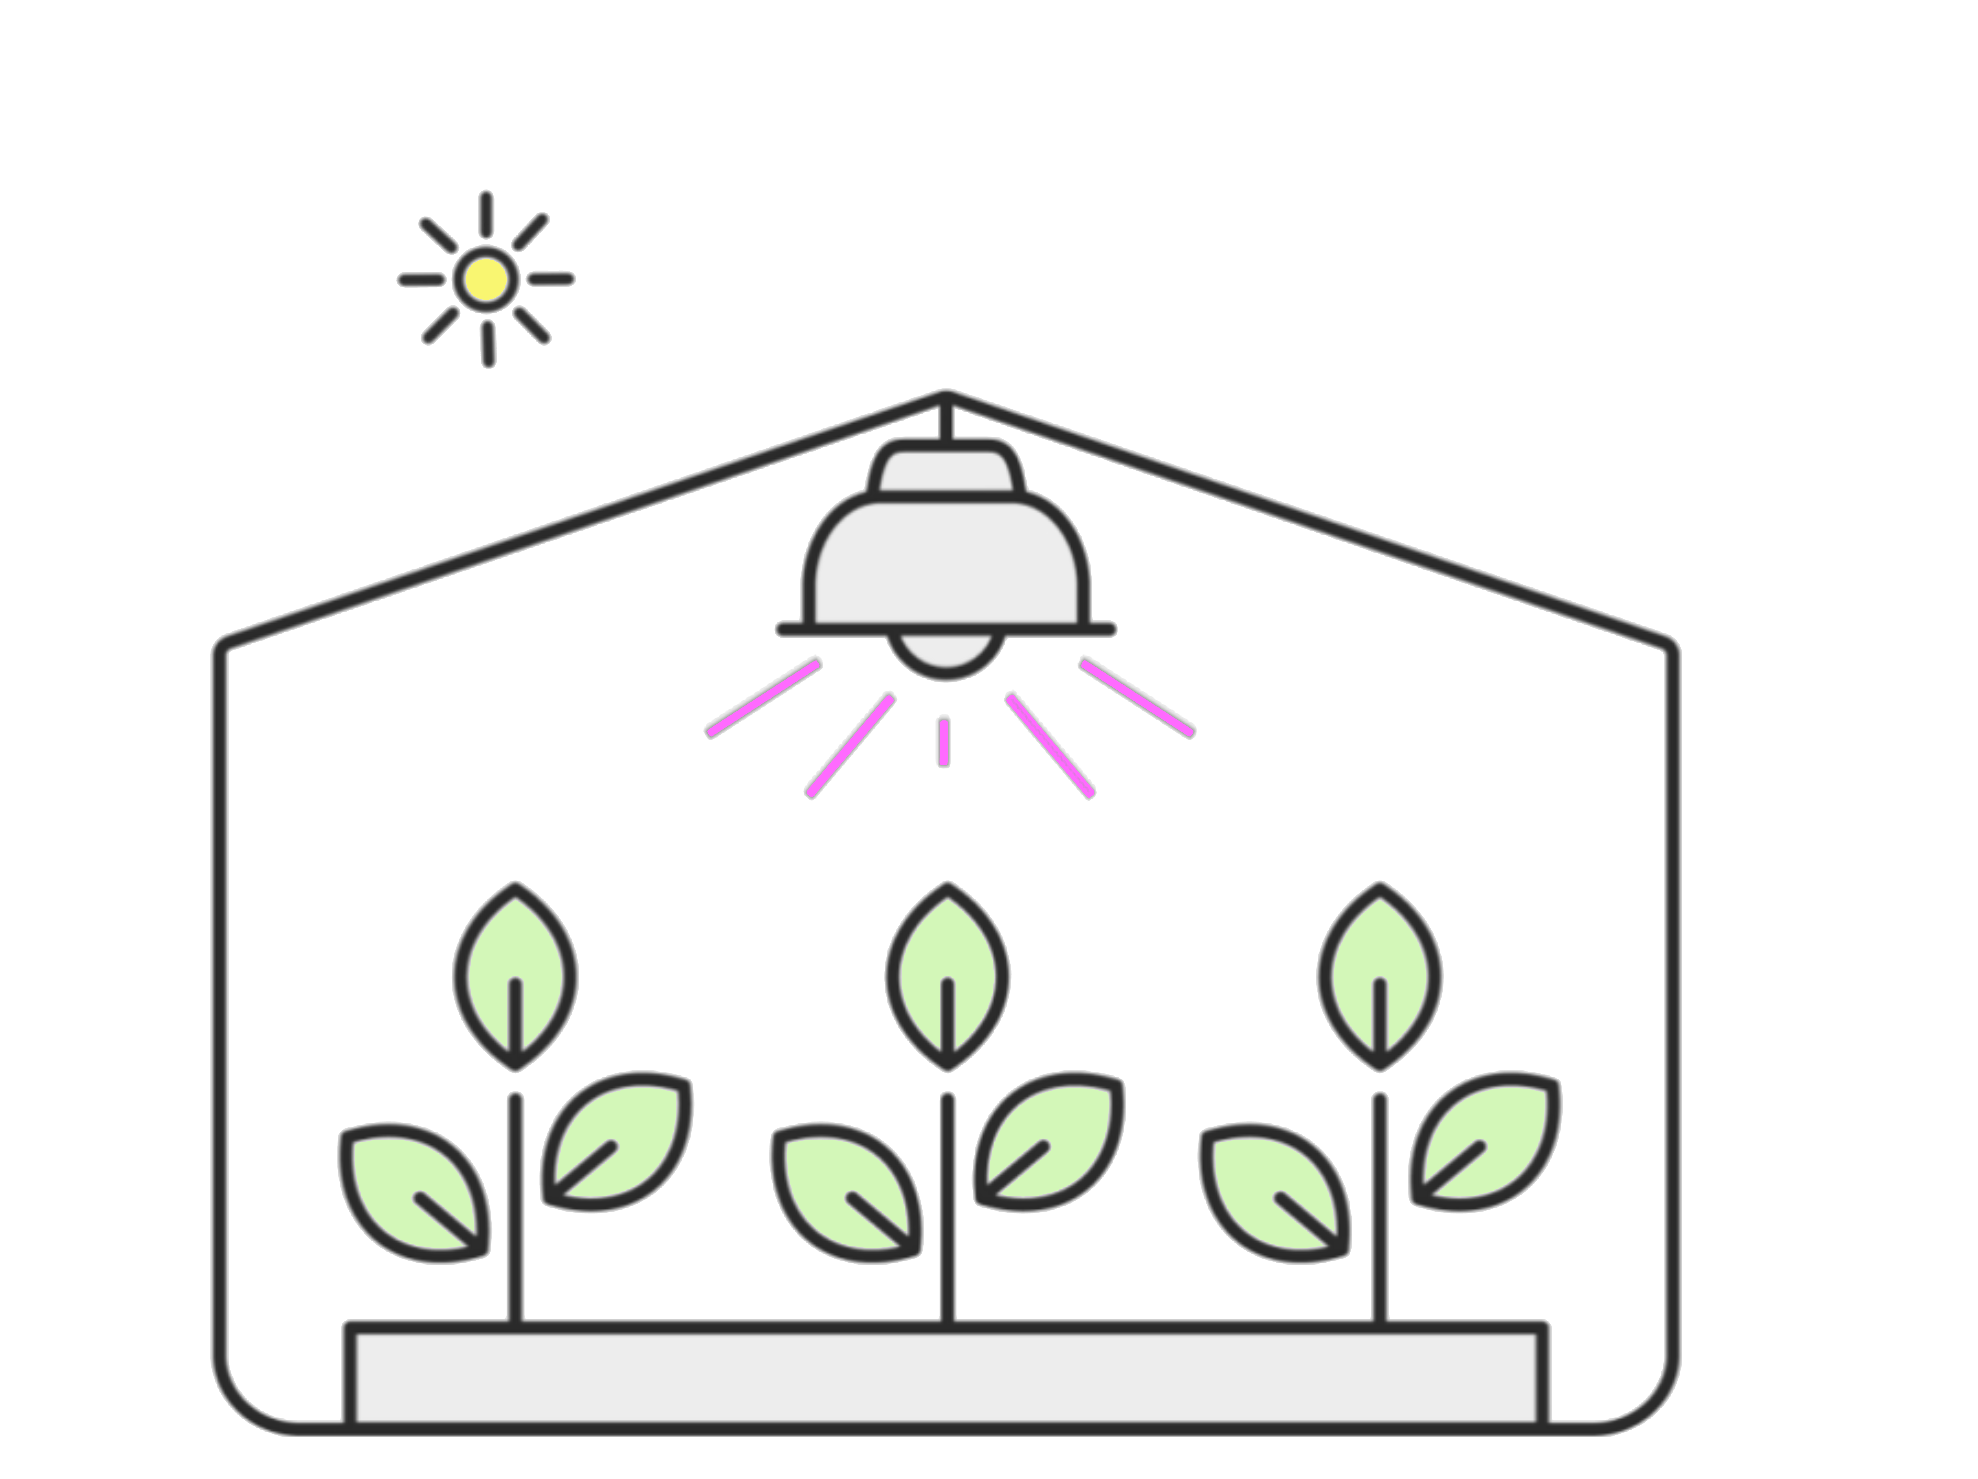
\includegraphics[scale=0.2]{figures/4_lights.png}
        \end{figure}
    }
    \only<7>{
        \begin{columns}
            \begin{column}{0.5\textwidth}
                \begin{figure}
                    \centering
                    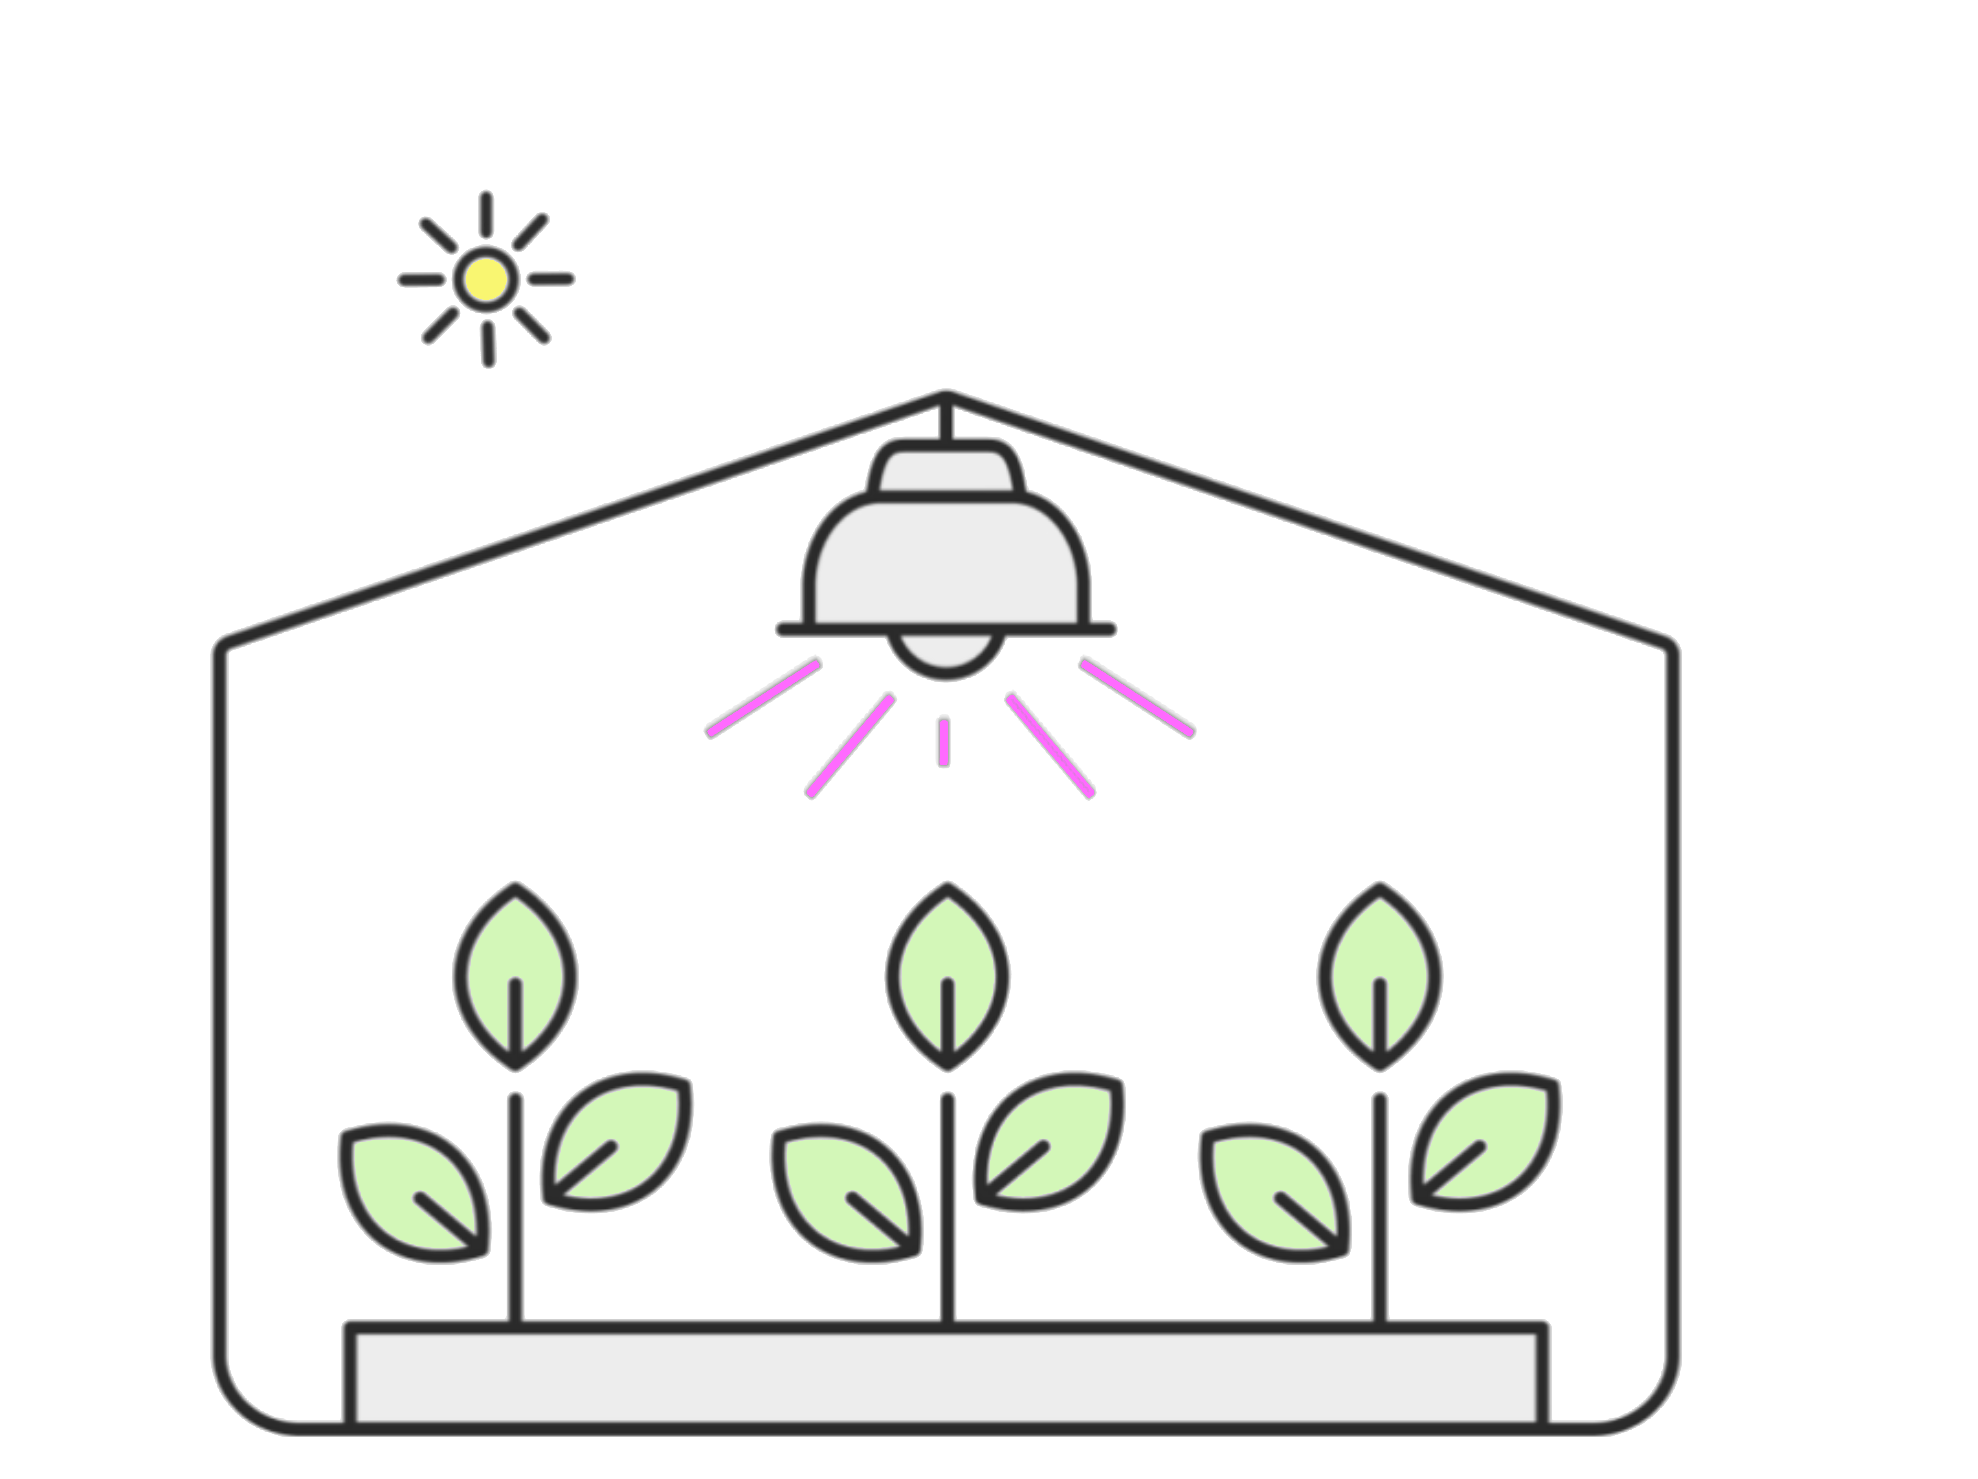
\includegraphics[scale=0.175]{figures/4_lights.png}
                \end{figure}
            \end{column}
            \begin{column}{0.5\textwidth}
                \begin{figure}
                    \centering
                    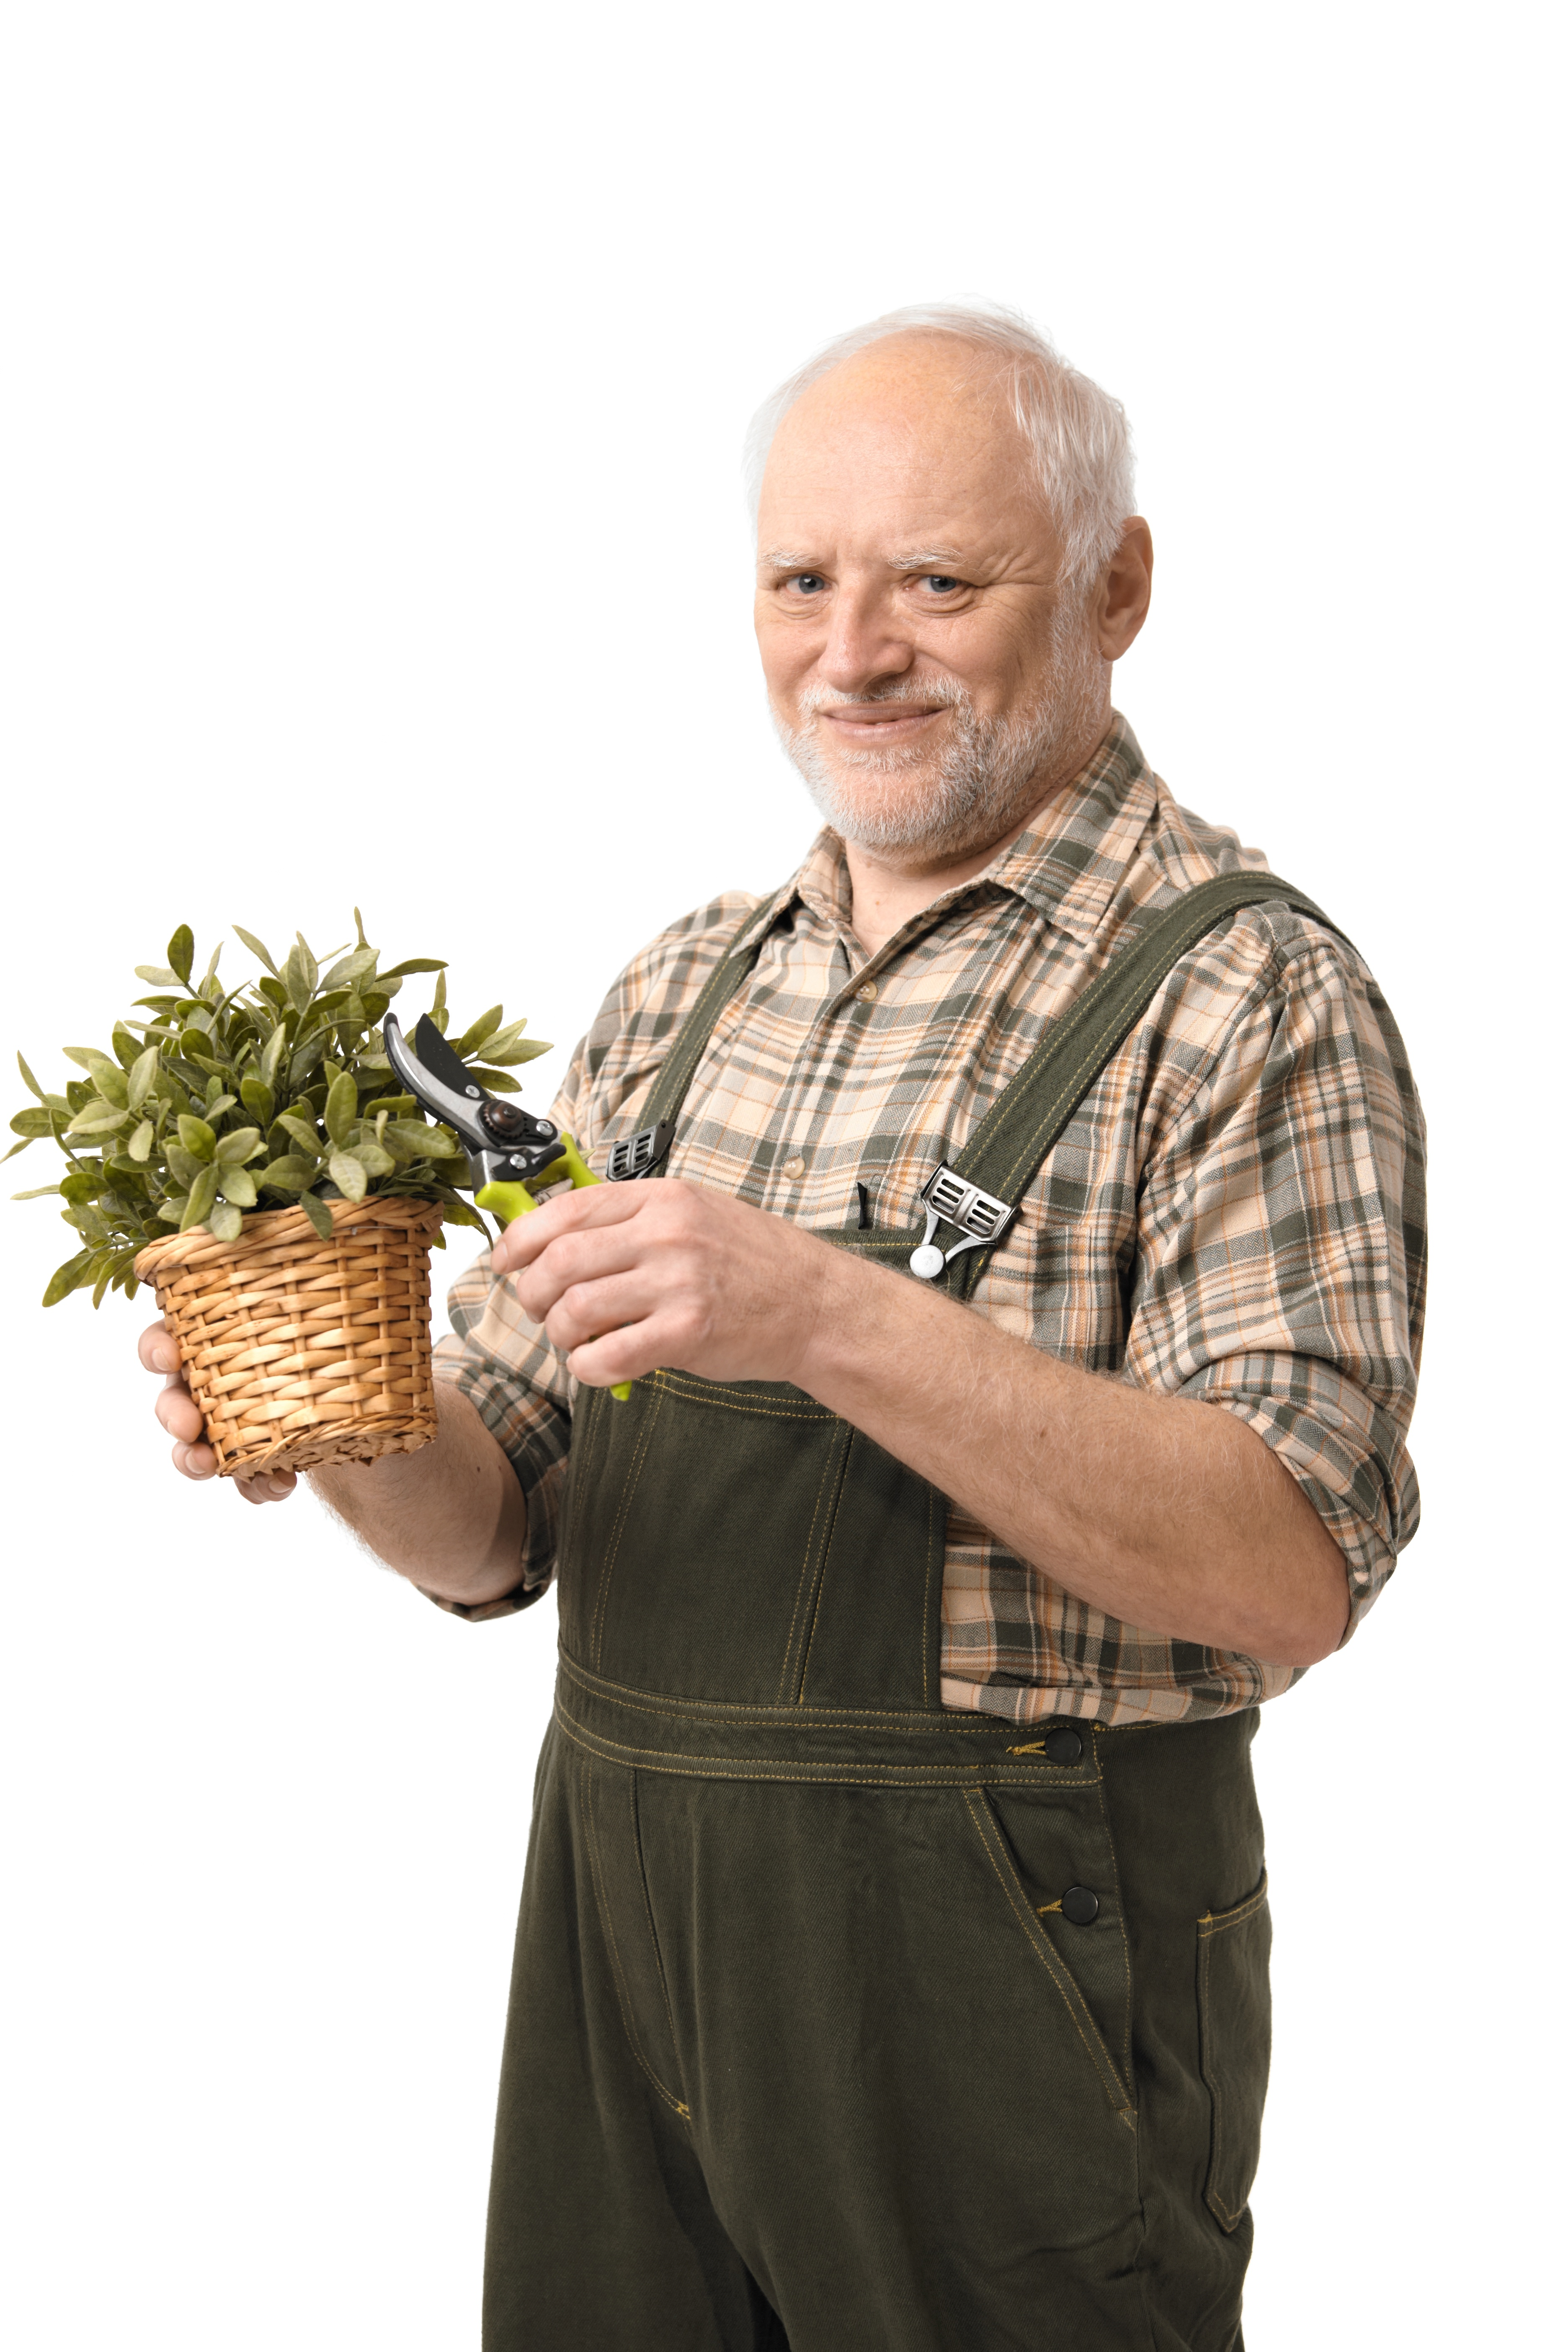
\includegraphics[scale=0.1]{figures/gardener.jpeg}
                \end{figure}
            \end{column}
        \end{columns}
    }
    \only<8>{
        \begin{columns}
            \begin{column}{0.5\textwidth}
                \begin{figure}
                    \centering
                    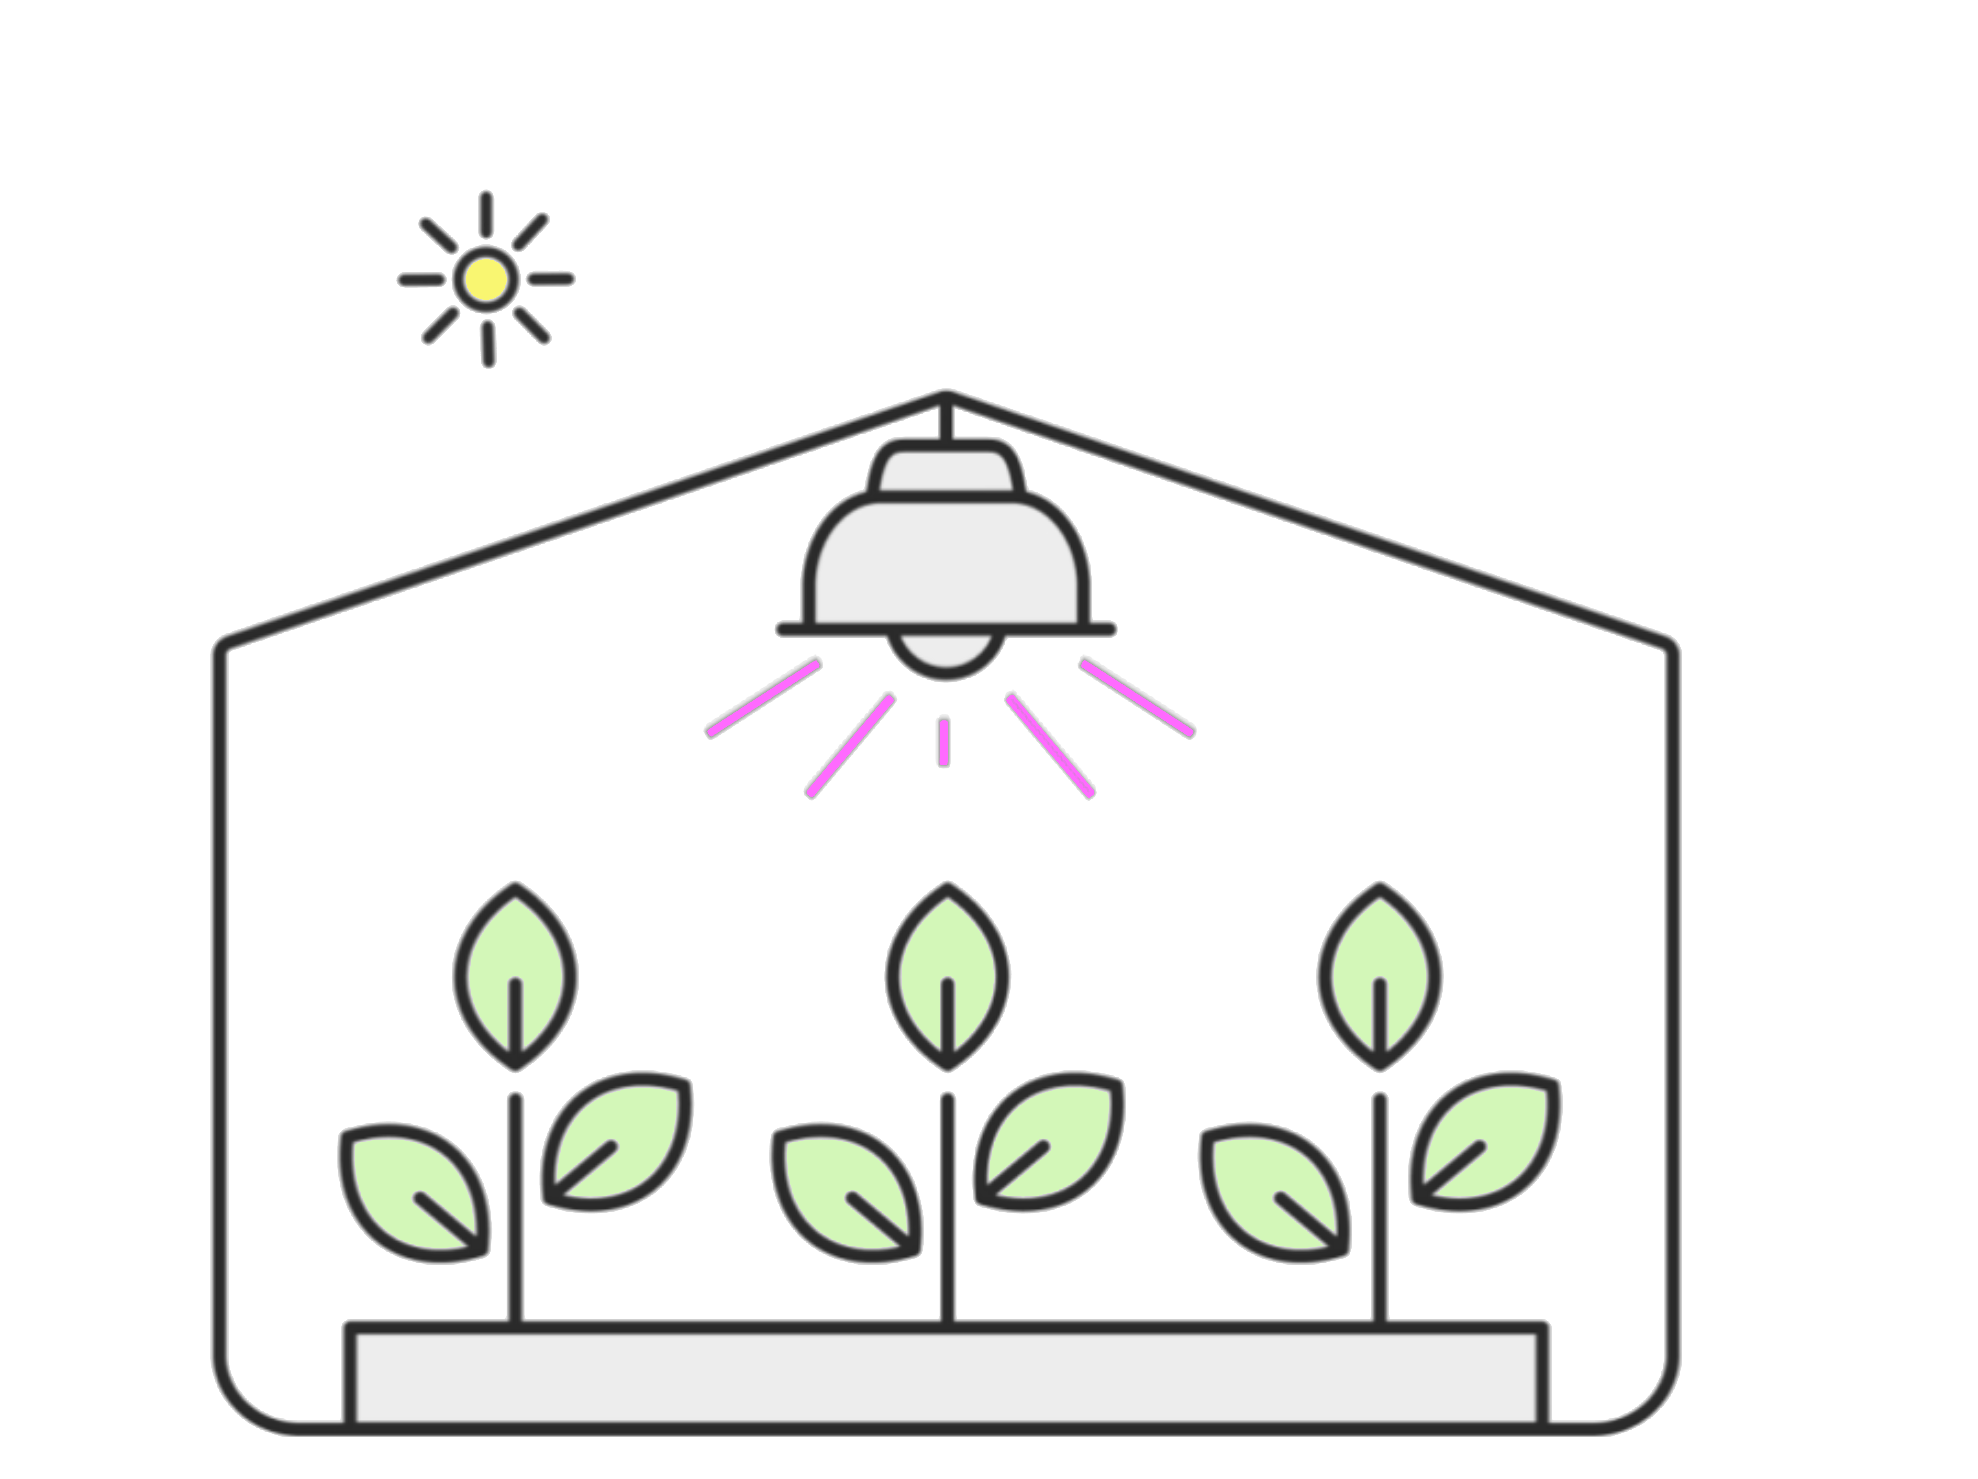
\includegraphics[scale=0.175]{figures/4_lights.png}
                \end{figure}
            \end{column}
            \begin{column}{0.5\textwidth}
                \begin{figure}
                    \centering
                    
\includegraphics[scale=0.1]{figures/computer.jpeg}
                \end{figure}
            \end{column}
        \end{columns}
    }
\end{frame}

\begin{frame}
    \frametitle{Model Predictive Control}
    
    \begin{figure}
        \centering
        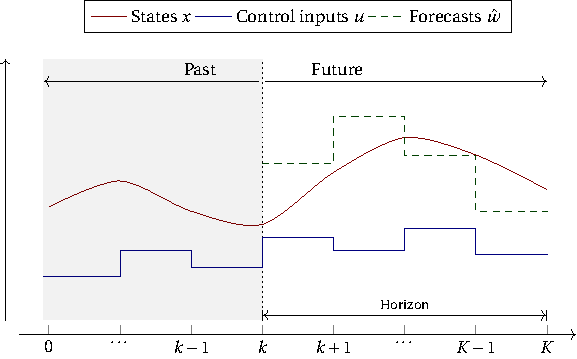
\includegraphics[scale=0.8]{figures/mpc1.pdf}
        \caption{Example trajectories of model predictive control scheme.}
    \end{figure}

\end{frame}